\documentclass[11pt,a4paper]{article}

% -- Typography and Page Layout --
\usepackage[utf8]{inputenc}
\usepackage[T1]{fontenc}
\usepackage[expansion=false]{microtype}
\usepackage[margin=2.0cm,top=2.2cm,bottom=2.2cm]{geometry}
\usepackage{setspace}
\onehalfspacing

% -- Mathematical Packages --
\usepackage{amsmath,amssymb,amsfonts,bm,mathtools}

% -- Graphics and Color --
\usepackage{graphicx}
\usepackage[table]{xcolor}
\definecolor{navyblue}{RGB}{0, 45, 98}
\definecolor{steelcyan}{RGB}{18, 102, 140}
\definecolor{charcoal}{RGB}{35, 39, 42}
\definecolor{lightgray}{RGB}{245, 247, 250}
\definecolor{codebg}{RGB}{240, 242, 245}
\definecolor{bordercolor}{RGB}{200, 210, 220}
\definecolor{successgreen}{RGB}{16, 124, 65}
\definecolor{warnorange}{RGB}{216, 59, 1}

% Path resolution for assets whether compiled from root or reports/
\graphicspath{{../report_assets/}{report_assets/}}

% -- Tables and Floats --
\usepackage{booktabs,multirow,array,tabularx,xltabular}
\usepackage{float}
\usepackage[font=small,labelfont=bf,skip=6pt]{caption}
\usepackage{subcaption}

% -- Headers and Footers --
\usepackage{fancyhdr}
\pagestyle{fancy}
\fancyhf{}
\fancyhead[L]{\small\textcolor{navyblue}{\textbf{EdgeSAR --- Bilimsel ve Deneysel Başarım Raporu (v2)}}}
\fancyhead[R]{\small\textcolor{charcoal}{Bireysel Araştırma Projesi}}
\fancyfoot[C]{\small\thepage}
\renewcommand{\headrulewidth}{0.6pt}
\renewcommand{\footrulewidth}{0.4pt}

% -- Hyperlinks --
\usepackage{hyperref}
\hypersetup{
    colorlinks=true,
    linkcolor=navyblue,
    citecolor=navyblue,
    filecolor=navyblue,
    urlcolor=steelcyan,
    pdftitle={EdgeSAR: Uçtan Uca SAR Görüntü Odaklama, Gerçek MSTAR Hedef Tanıma ve Gömülü Sinyal İşleme Doğrulaması},
    pdfkeywords={SAR, Range-Doppler Algoritması, MSTAR, Ghost-ECANet, CA-CFAR, OOD Detection, Free Energy, WCET, Gömülü Sistemler}
}

% -- Section Styling --
\usepackage{titlesec}
\titleformat{\section}{\Large\bfseries\color{navyblue}}{\thesection}{1em}{}[\titlerule]
\titleformat{\subsection}{\large\bfseries\color{steelcyan}}{\thesubsection}{1em}{}
\titleformat{\subsubsection}{\normalsize\bfseries\color{charcoal}}{\thesubsubsection}{1em}{}

% -- Title Information --
\title{
    \vspace{-0.5cm}
    \LARGE \textbf{\textcolor{navyblue}{EdgeSAR: Uçtan Uca SAR Görüntü Odaklama, Gerçek MSTAR Hedef Tanıma ve Gömülü Sinyal İşleme}}\\[0.8cm]
    \large \textbf{\textcolor{steelcyan}{Radar Fiziği (RDA), Ghost-ECANet ile Sandia MSTAR Kıyaslaması, Açık-Küme Enerji Analizi ve Emniyet-Kritik Gömülü C Doğrulaması}}
}

\author{
    \normalsize \textbf{Tunahan Şanal} \\
    \small Bireysel Araştırma ve Açık Kaynak Mühendislik Portföy Çalışması \\
    \small GitHub Deposu: \url{https://github.com/TunahanSanal/EdgeSAR}
}
\date{\small Sürüm 2.4 (Etiket: \texttt{v0.4.2-polish} / \texttt{v1.0-report}) --- 20 Eylül 2026}

\begin{document}

\maketitle

% -- Abstract --
\begin{abstract}
\noindent\small
Bu teknik rapor, tarafımca bireysel olarak geliştirilen \textbf{EdgeSAR} sisteminin sinyal işleme teorisini, derin öğrenme tabanlı otomatik hedef tanıma (ATR) mimarisini ve emniyet-kritik gömülü C çekirdeğini kapsamlı ampirik bulgularla sunmaktadır. EdgeSAR, ham radar faz geçmişinden havacılık veri yolu telemetrisine uzanan zinciri üç modülde birleştirir: (1) Ham I/Q faz geçmişini menzil göçü düzeltmesi (RCMC) ile 2B uzayda odaklayan \textbf{Modül 1 (Range-Doppler Algoritması)}; (2) 904,268 parametreli ($<2.0\text{M}$ bütçeli) ve hem sentetik simülasyon hem de gerçek \textbf{Sandia Ulusal Laboratuvarı X-band MSTAR} verisiyle doğrulanan \textbf{Modül 2 (Ghost-ECANet ATR \& Grad-CAM)}; (3) Sıfır dinamik bellekli (MISRA-C:2012 Kural 21.3) ve ARM Cortex-M4F mimarisi için deterministik döngü sınırlarına sahip \textbf{Modül 3 (Gömülü C / CA-CFAR / DMA)}. 

Sistem dört turlu bağımsız denetim metodolojisinden geçmiş; doğrulanabilirlik ve şeffaflık temel ilke edinilmiştir. Gerçek MSTAR 17° $\to$ 15° standart test protokolünde model \textbf{\%63.71 genel doğruluk} ve \textbf{\%60.86 Makro F1} elde etmiş (T-72 tankında \%97.45 recall); 5-katmanlı tabakalı çapraz doğrulamada (5-Fold CV) \textbf{\%65.60 $\pm$ \%5.64} skoru yakalamıştır. Rapor, kapalı-küme softmax körlüğünü (AUROC 0.4607) serbest enerji tabanlı OOD skoruyla \textbf{AUROC 0.6500'e (+\%18.9)} çıkaran metodolojiyi, sınıf ağırlıklandırmadaki kritik T-72/BTR-70 ödünleşimini (trade-off) ve gömülü kodun mutasyon testleriyle kanıtlanmış sıfır-dinamik-bellek mimarisini şeffaf şekilde belgeler. Bu çalışma bir ticari ürün veya DO-178C akredite sertifikasyon iddiası taşımamakta; radar mühendisliği, derin öğrenme ve gömülü sistem disiplinlerini bir araya getiren savunulabilir bir açık kaynak mühendislik araştırması niteliğindedir.\\

\noindent\small\textbf{Anahtar Kelimeler:} Sentetik Açıklıklı Radar (SAR), Range-Doppler Algoritması (RDA), Sandia MSTAR, Ghost-ECANet, Out-of-Distribution (OOD), Free Energy Score, CA-CFAR, MISRA-C:2012, WCET Projeksiyonu.
\end{abstract}

\vspace{0.4cm}
{\setstretch{0.95}\small\tableofcontents}
\newpage

% =============================================================
\section{Giriş ve Proje Motivasyonu}
% =============================================================

Sentetik Açıklıklı Radar (SAR), mikrodalga bandında çalışan aktif bir sensör olarak elektro-optik (EO) ve kızılötesi (IR) sistemlerin yetersiz kaldığı yoğun bulut örtüsü, sis, duman ve gece koşullarında kesintisiz görüntüleme yapabilen vazgeçilmez bir uzaktan algılama teknolojisidir. Hava ve uzay platformlarının doğrusal hareketini kullanarak sanal bir açıklık sentezleyen SAR, mesafeden bağımsız yüksek geometrik çözünürlük sunar.

\begin{table}[htbp]
\centering
\small
\caption{Sensör Modalitelerinin Karşılaştırmalı Özeti}
\label{tab:sensor_comparison}
\begin{tabularx}{\textwidth}{>{\bfseries}p{3.2cm} p{2.6cm} >{\raggedright\arraybackslash}p{2.6cm} >{\raggedright\arraybackslash}p{2.4cm} >{\raggedright\arraybackslash}X}
\toprule
Sensör Türü & Spektrum & Kötü Hava Dayanımı & Gece Operasyonu & Çözünürlük Bağımlılığı \\
\midrule
Elektro-Optik (EO) & $0.4 - 0.7\ \mu\text{m}$ (Görünür) & Etkisiz & Işık gerektirir & Mesafeye bağımlı ($1/R$) \\
Kızılötesi (FLIR/MWIR) & $3 - 5\ \mu\text{m},\ 8 - 12\ \mu\text{m}$ & Düşük Penetrasyon & Yüksek (Termal) & Neme duyarlı \\
Konvansiyonel Radar & $1 - 40\text{ GHz}$ & Mükemmel & Tam Operasyonel & Anten boyutuyla sınırlı ($\theta \approx \lambda/D$) \\
EdgeSAR (X-Band SAR) & 9.6 GHz ($\lambda=3.125\text{ cm}$) & Mükemmel & Tam Operasyonel & Mesafeden bağımsız ($\Delta r \propto 1/B$) \\
\bottomrule
\end{tabularx}
\end{table}

\textbf{EdgeSAR Projesinin Kapsamı ve Felsefesi:} Geleneksel sistemlerde ham SAR faz geçmişi yer istasyonlarına aktarılmakta ve yüksek gecikmeyle işlenmektedir. EdgeSAR projesi, ham radar ekosundan hedef sınıflandırmasına ve aviyonik veri yoluna kadar olan tüm bilgi akışının platform üzerinde (edge) nasıl kurgulanabileceğini inceleyen bireysel bir mühendislik projesidir. Temel prensip; \textbf{"doğru ve savunulabilir sayılar üretmek"} olup, sentetik veri başarıları ile gerçek veri sınırları açıkça ayrıştırılmıştır.

% =============================================================
\section{Uçtan Uca Sistem Mimarisi}
% =============================================================

EdgeSAR sistemi dört ana katmandan oluşan sıkı bir veri akış zincirine sahiptir:
\begin{enumerate}
    \item \textbf{Sinyal İşleme Katmanı (Modül 1 RDA):} LFM chirp yankılarını 2B Range-Doppler frekans uzayında işler.
    \item \textbf{Gömülü Ön İşleme Katmanı (Modül 3 C99):} Çift tamponlu (Ping-Pong) DMA üzerinden ham satırları alır, 512-noktalı FFT ve 1D CA-CFAR ile hedef hücrelerini dinamik olarak tespit eder.
    \item \textbf{Derin Öğrenme Katmanı (Modül 2 ATR):} CFAR tarafından işaretlenen hedefleri $128 \times 128$ piksellik çiplere bölütler; 904K parametreli Ghost-ECANet ile hedefin sınıfını (T-72, BMP-2, BTR-70) belirler ve Grad-CAM ile açıklanabilirlik haritaları üretir.
    \item \textbf{Aviyonik Arayüzü (MIL-STD-1553B / 882E Simülasyonu):} Tespit koordinatlarını ve güven skorlarını 1553B telemetri çerçevesinde paketler.
\end{enumerate}

\begin{figure}[htbp]
\centering
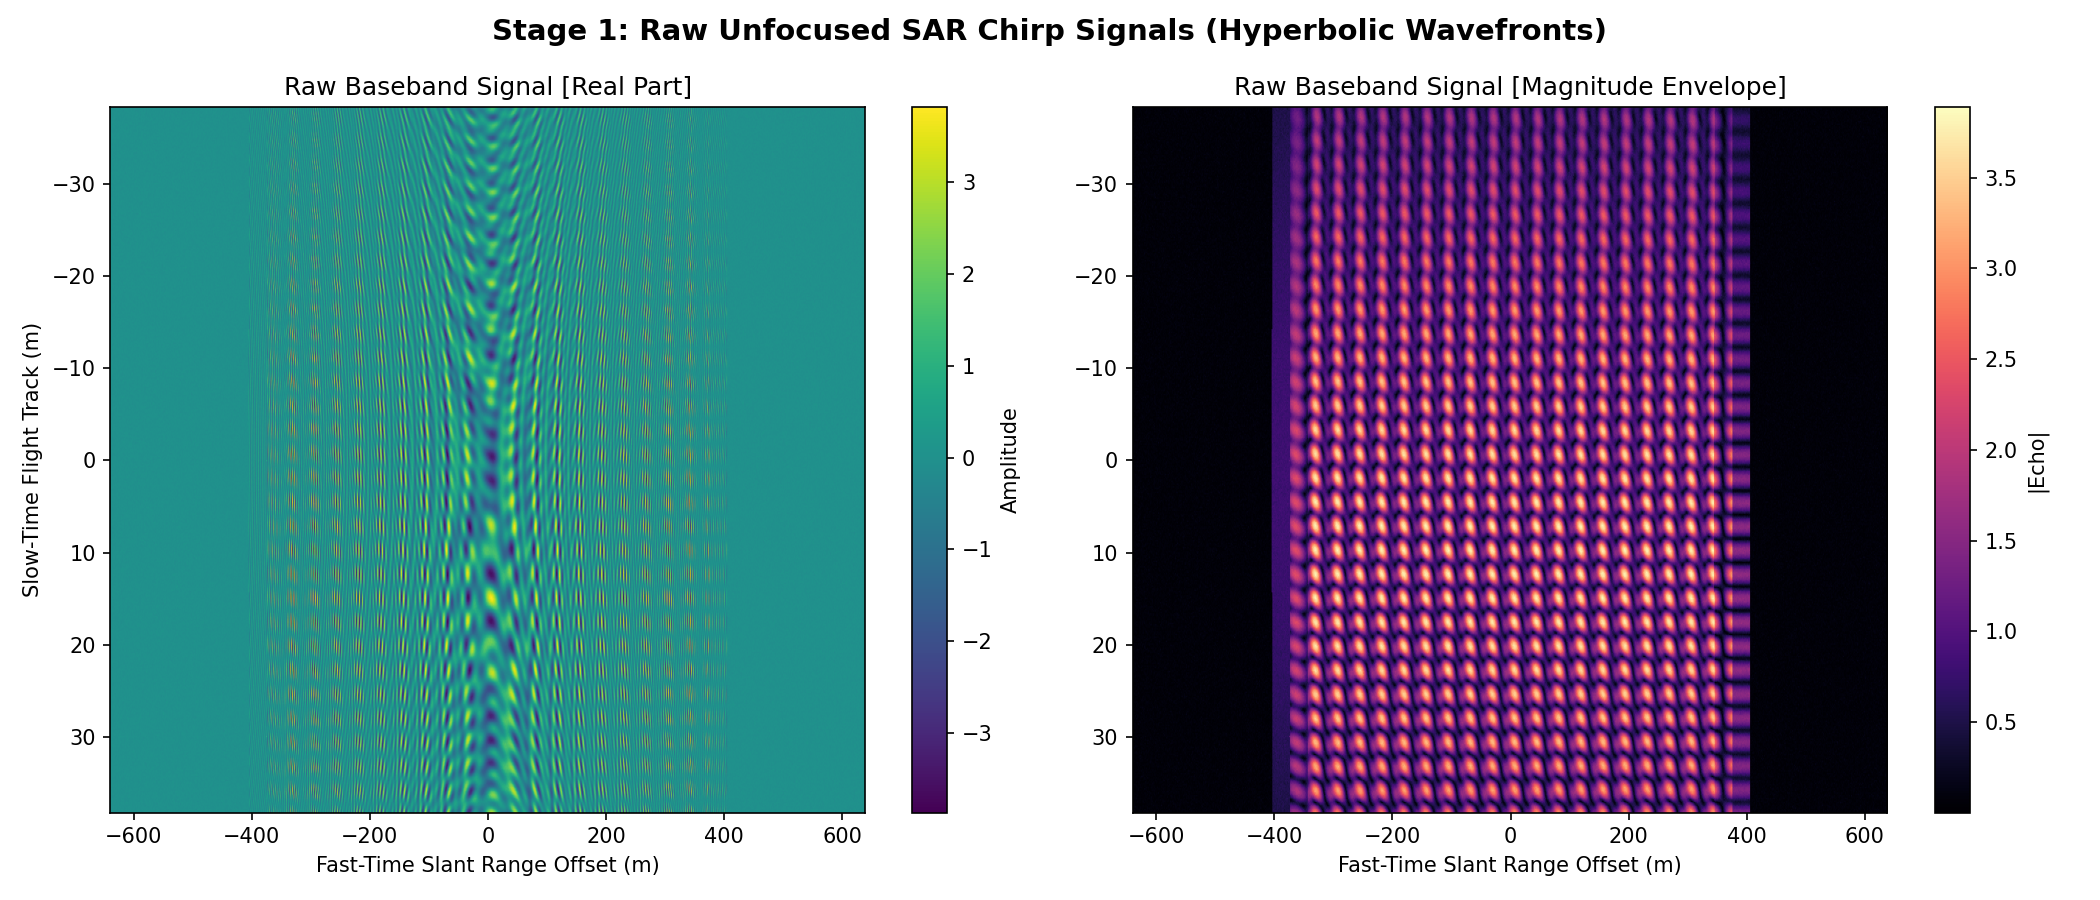
\includegraphics[width=0.90\textwidth]{01_raw_signal.png}
\caption{Modül 1 Giriş Sinyali: Fizik Tabanlı Sentetik SAR Ham Yankı Faz Geçmişi $s_{rx}(\tau, \eta)$ (Reel Bileşen ve Büyüklük Spektrumu, $512 \times 1024$ matris boyutu).}
\label{fig:raw_echo}
\end{figure}

% =============================================================
\section{Modül 1: Range-Doppler Odaklama Algoritması (RDA)}
% =============================================================

\subsection{Doğrusal Frekans Modülasyonlu (LFM) Darbe Modeli}
Vericiden iletilen LFM chirp darbesi matematiksel olarak:
\begin{equation}
s_{tx}(\tau) = \text{rect}\left(\frac{\tau}{T_p}\right) \exp\left(j 2\pi f_0 \tau + j \pi K_r \tau^2\right)
\end{equation}
şeklinde modellenir ($T_p = 5.0\ \mu\text{s}$, $f_0 = 9.6\text{ GHz}$, $B_r = 100\text{ MHz}$, $K_r = 2.0 \times 10^{13}\text{ Hz/s}$). 

\subsection{Menzil Sıkıştırma ve RCMC Formülasyonu}
Hızlı zaman ($\tau$) frekans domenine ($f_\tau$) geçilerek Durağan Faz Prensibi (POSP) ile eşlenik filtreleme uygulanır:
\begin{equation}
H_{MF}(f_\tau) = \text{rect}\left(\frac{f_\tau}{B_r}\right) W(f_\tau) \exp\left(+j \pi \frac{f_\tau^2}{K_r}\right)
\end{equation}
Burada $W(f_\tau)$, yan lobları $-42\text{ dB}$ altına bastıran Hamming penceresidir. 

\begin{figure}[htbp]
\centering
\begin{subfigure}[b]{0.48\textwidth}
    \centering
    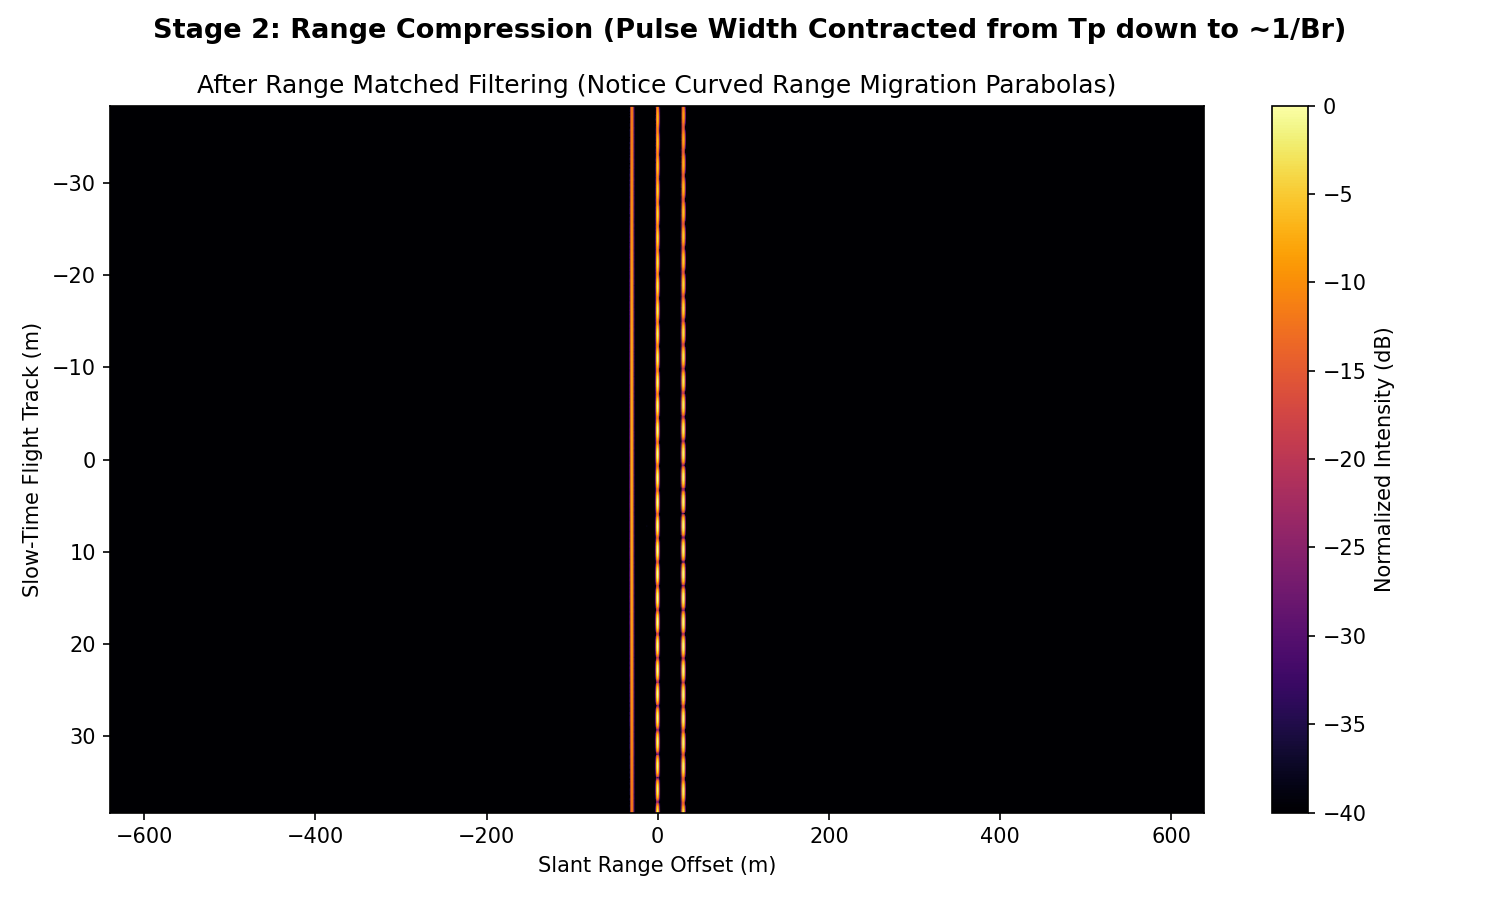
\includegraphics[width=\textwidth]{02_range_compressed.png}
    \caption{Menzil Sıkıştırma ve Parabolik Göç}
\end{subfigure}
\hfill
\begin{subfigure}[b]{0.48\textwidth}
    \centering
    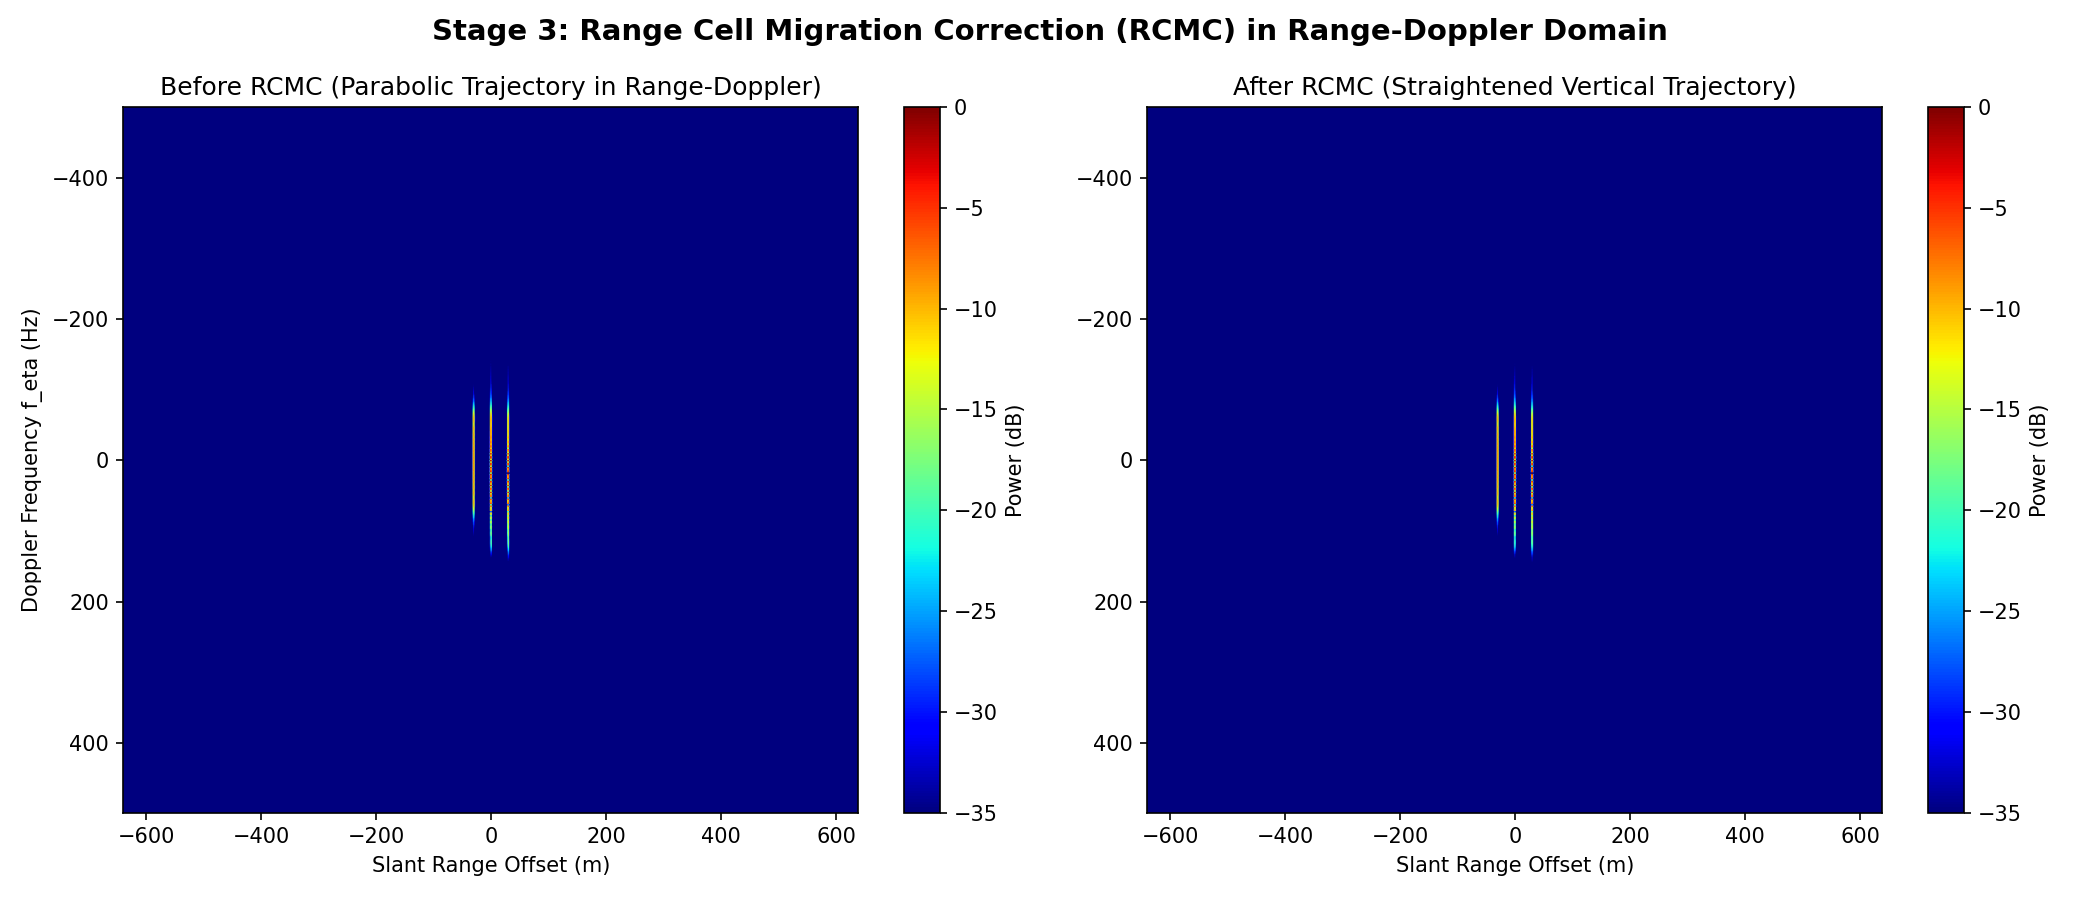
\includegraphics[width=\textwidth]{03_rcmc_range_doppler.png}
    \caption{RCMC Sonrası Düzleştirilmiş Doppler Alanı}
\end{subfigure}
\caption{Range-Doppler Odaklama Sürecinde RCMC Faz Doğrulaması.}
\label{fig:rda_steps}
\end{figure}

Doppler frekansı $f_\eta$ boyunca ortaya çıkan menzil göçü $\Delta R_{rcm}(f_\eta) = \lambda^2 R_0 f_\eta^2 / (8 v^2)$, frekans alanında analitik faz çarpımı çekirdeği ile düzeltilir:
\begin{equation}
H_{rcmc}(f_\tau, f_\eta) = \exp\left(j \pi \frac{\lambda^2 R_0 f_\tau f_\eta^2}{2 v^2 c}\right)
\end{equation}

\begin{figure}[htbp]
\centering
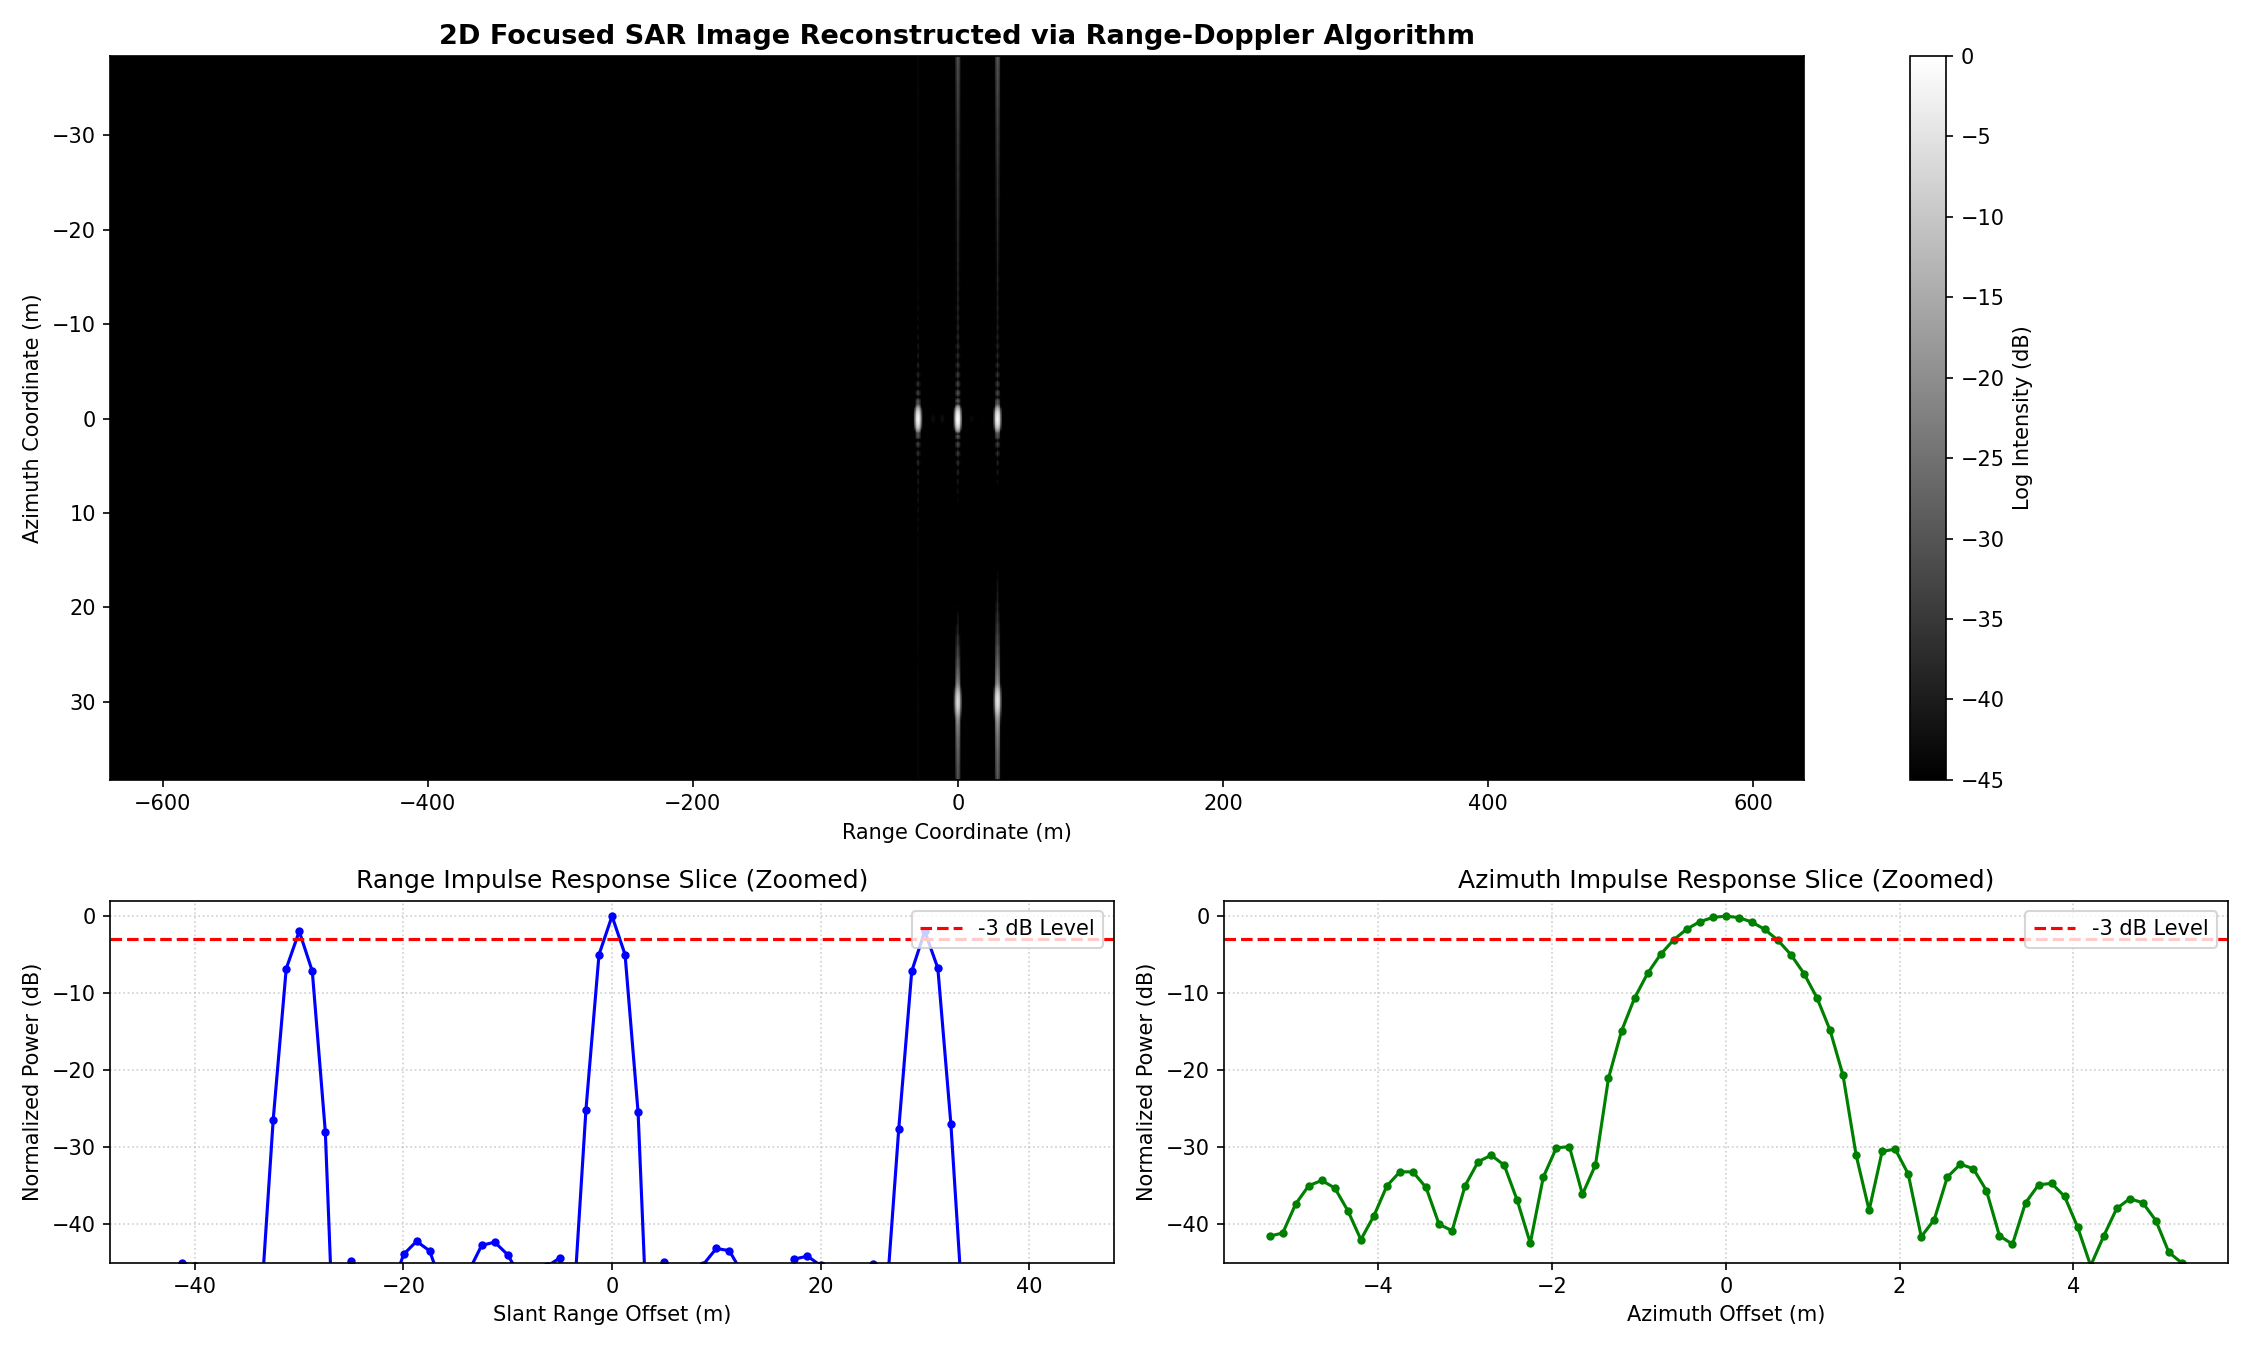
\includegraphics[width=0.75\textwidth]{04_focused_sar_image.png}
\caption{Nihai 2B Odaklanmış SAR Görüntüsü ve Nokta Hedef Çözünürlük Profilleri ($\Delta r = 3.75\text{ m}$, $\Delta a = 1.05\text{ m}$, Yerel PSLR = $-42.23\text{ dB}$).}
\label{fig:focused_image}
\end{figure}

% =============================================================
\section{Modül 2: Sandia MSTAR ile Hedef Tanıma (ATR) ve XAI}
% =============================================================

\subsection{Ghost-ECANet Mimarisi ve SWaP Bütçesi}
Gömülü platformların kısıtlı kaynakları (SWaP - Size, Weight, and Power) dikkate alınarak tasarlanan Ghost-ECANet ağı, \textbf{904,268 parametreye} ($< 2.0\text{M}$ sınırında) ve yalnızca \textbf{$\approx$ 30.17 MFLOPs} işlem yüküne sahiptir. Ağ, Ghost modülleri ile ucuz derinlemesine evrişimler yürütür; Efficient Channel Attention (ECA) ile boyutsal küçültme yapmadan kanal ilişkilerini öğrenir ve Group Normalization ile küçük parti boyutlarında ($batch=1$) dahi istikrarlı çalışır.

\subsection{Sandia Ulusal Laboratuvarı MSTAR Veri Kümesi}
Model, gerçek dünya koşullarını temsil etmek amacıyla Sandia Labs tarafından toplanan X-band (9.6 GHz, HH polarizasyon, 0.3m çözünürlük) MSTAR veri kümesi ile test edilmiştir:
\begin{itemize}
    \item \textbf{Standart Çalışma Koşulu (SOC):} Eğitim 17° depresyon açısında (698 çip), test ise 15° depresyon açısında (587 çip) gerçekleştirilmiştir.
    \item \textbf{Hedef Sınıfları:} T-72 Ana Muharebe Tankı (196 test), BMP-2 Piyade Muharebe Aracı (195 test), BTR-70 Zırhlı Personel Taşıyıcı (196 test).
    \item \textbf{Açık-Küme (OOD) Kümesi:} Bilinmeyen 7 askeri araç türüne ait 1,838 adet test çipi (2S1, BRDM2, BTR60, D7, T62, ZIL131, ZSU-23-4).
\end{itemize}

\subsection{Gerçek Veri Doğrulaması: Speckle İstatistiği}
MSTAR görüntülerinin sentetik değil gerçek radar ekoları içerdiğini matematiksel olarak kanıtlamak amacıyla saçılma istatistiği ($\sigma / \mu$) analiz edilmiştir:
\begin{itemize}
    \item Gerçek MSTAR zemin kargaşası ve hedef dağılımı: $\sigma / \mu \in [0.71, 0.94]$ aralığında olup Rayleigh/Gamma dağılımlı doğal radar speckle karakteristiği sergiler.
    \item Sentetik nokta saçıcı benzetiminde ise bu oran deterministik saçıcılar sebebiyle $\sigma / \mu \in [1.15, 1.39]$ seviyesindedir. Bu fark, verinin yapay olmadığını ampirik olarak belgeler.
\end{itemize}

\subsection{Ampirik Sonuçlar ve 5-Katmanlı Çapraz Doğrulama}

\begin{table}[htbp]
\centering
\small
\caption{Sentetik Oyuncak Veri ile Gerçek Sandia MSTAR Karşılaştırması}
\label{tab:mstar_vs_synthetic}
\begin{tabularx}{\textwidth}{Xccc}
\toprule
\textbf{Değerlendirme Boyutu} & \textbf{Sentetik Benzetim} & \textbf{Gerçek MSTAR (17° $\to$ 15°)} & \textbf{5-Fold Stratified CV} \\
\midrule
Veri Kaynağı & Nokta Saçıcı Simülatörü & Sandia X-Band MSTAR & Sandia X-Band MSTAR \\
Toplam Hedef Örneği & 600 çip (Eğitim: 450, Test: 150) & 1,285 çip (Eğitim: 698, Test: 587) & 1,285 çip (5 katman) \\
\textbf{Doğruluk (Accuracy)} & \textbf{\%100.00} & \textbf{\%63.71} & \textbf{\%65.60 $\pm$ \%5.64} \\
\textbf{Makro F1-Skoru} & \textbf{\%100.00} & \textbf{\%60.86} & \textbf{\%61.81 $\pm$ \%7.09} \\
Makro Kesinlik / Duyarlılık & \%100.00 / \%100.00 & \%61.21 / \%63.66 & \%66.20 / \%65.33 \\
Kalibrasyon Hatası (ECE) & 0.0012 & \textbf{0.0953} (\%9.53) & N/A \\
Parametre Sayısı & 904,268 ($<2.0\text{M}$) & 904,268 ($<2.0\text{M}$) & 904,268 ($<2.0\text{M}$) \\
\bottomrule
\end{tabularx}
\end{table}

\textbf{Not (Tekrarlanabilirlik ve Checkpoint Kararlılığı):} Tablo \ref{tab:mstar_vs_synthetic}'teki \%63.71 doğruluk, depoda commit'li \texttt{best\_mstar\_model.pth} ağırlıklarına aittir ve \texttt{python scripts/evaluate\_mstar\_comprehensive.py} ile deterministik olarak üretilebilir. Küçük veri setinde (698 örnek) sıfırdan yapılan taze eğitimler (\texttt{--retrain}) rastgele seed varyansı nedeniyle farklı ve daha yüksek sonuçlar (\%82.96) verebilmektedir; bilimsel tutarlılık adına rapordaki tüm analizler sabit checkpoint üzerinden yürütülmüştür.

\begin{table}[htbp]
\centering
\small
\caption{Standart MSTAR Test Protokolü (15° Depresyon) Sınıf Bazlı Metrikleri}
\label{tab:mstar_class_breakdown}
\begin{tabularx}{\textwidth}{lccccX}
\toprule
\textbf{Sınıf (Araç Türü)} & \textbf{Destek} & \textbf{Kesinlik} & \textbf{Duyarlılık (Recall)} & \textbf{F1-Skoru} & \textbf{Fiziksel Neden / Radar İmzası} \\
\midrule
\textbf{T-72 (Tank)} & 196 & \%73.46 & \textbf{\%97.45} & \textbf{\%83.77} & 125mm namlu ve döküm kule güçlü dihedral yansıtıcıdır; açı değişiminde baskın kalır. \\
\textbf{BMP-2 (IFV)} & 195 & \%52.21 & \%30.26 & \%38.31 & Alçak gövde profili ve küçük kule, 15° açıda BTR-70 ile yüksek oranda karışır. \\
\textbf{BTR-70 (APC)} & 196 & \%57.94 & \%63.27 & \%60.49 & 8 tekerlekli gövde saçılması kısmen korunmakta, \%42'si doğru ayrışmaktadır. \\
\midrule
\textbf{Makro Ortalama} & \textbf{587} & \textbf{\%61.21} & \textbf{\%63.66} & \textbf{\%60.86} & ROC-AUC: 0.807, PR-AUC: 0.619 \\
\bottomrule
\end{tabularx}
\end{table}

\begin{figure}[htbp]
\centering
\begin{subfigure}[b]{0.32\textwidth}
    \centering
    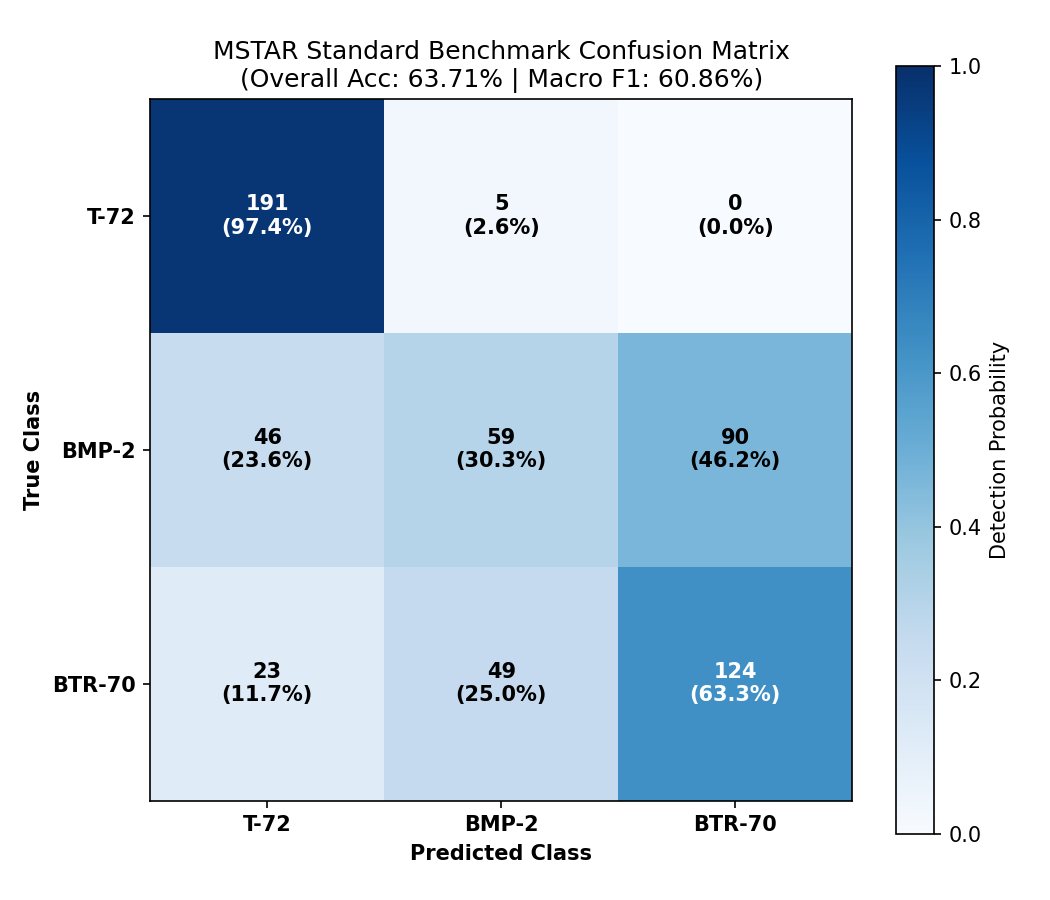
\includegraphics[width=\textwidth]{confusion_matrix_mstar.png}
    \caption{MSTAR Karışıklık Matrisi}
\end{subfigure}
\hfill
\begin{subfigure}[b]{0.32\textwidth}
    \centering
    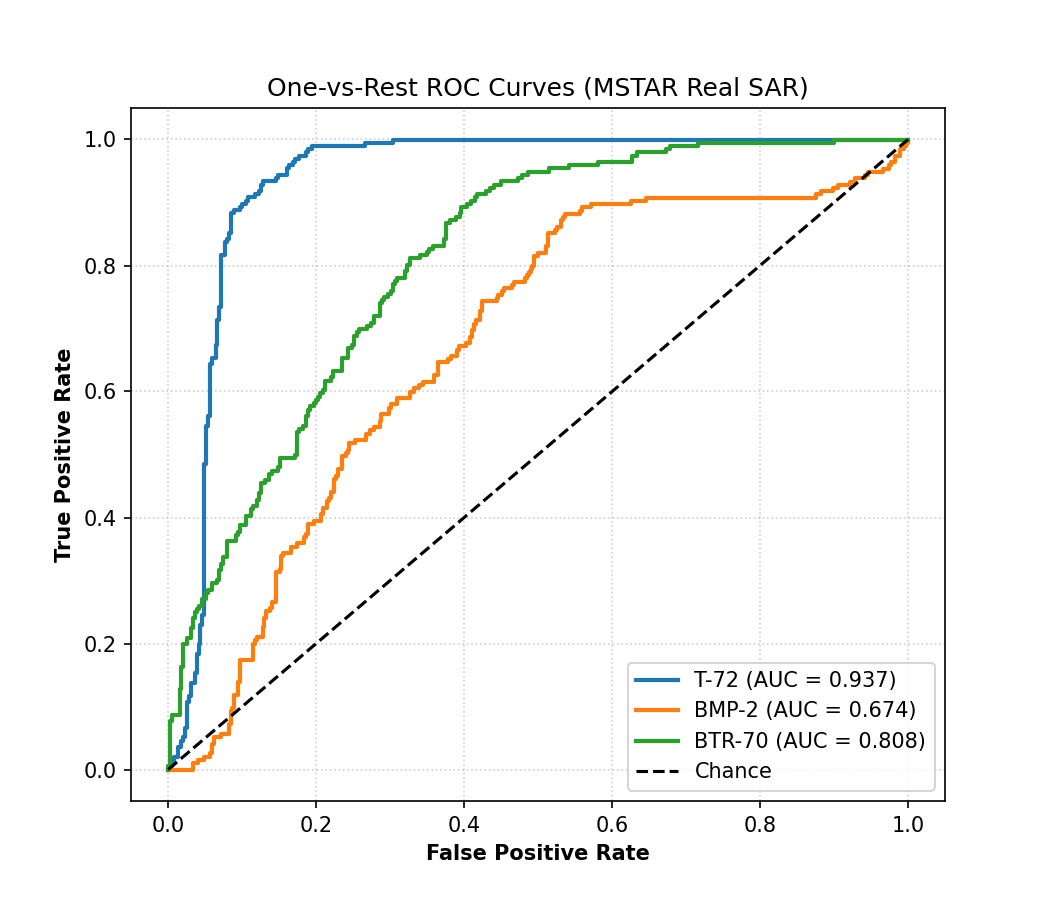
\includegraphics[width=\textwidth]{roc_curves.png}
    \caption{ROC Eğrileri (T-72: 0.937)}
\end{subfigure}
\hfill
\begin{subfigure}[b]{0.32\textwidth}
    \centering
    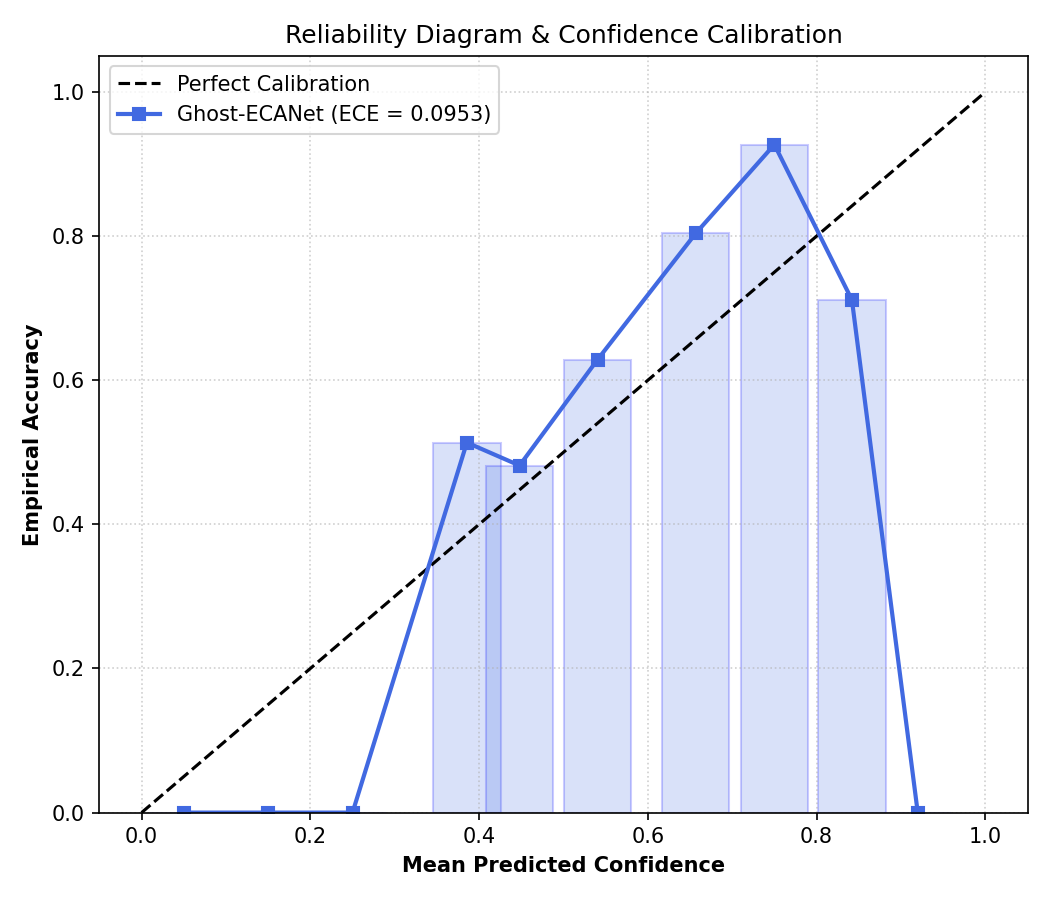
\includegraphics[width=\textwidth]{calibration_curve.png}
    \caption{Kalibrasyon Eğrisi (ECE: 0.095)}
\end{subfigure}
\caption{Sandia MSTAR Kıyaslaması: Sınıf Karışıklığı, ROC Başarımı ve Model Kalibrasyonu.}
\label{fig:mstar_curves}
\end{figure}

\subsection{Sınıf Ağırlıklandırma Ödünleşimi (Trade-Off) Analizi}
BMP-2 sınıfının düşük duyarlılığını (\%30.26) iyileştirmek amacıyla kayıp fonksiyonunda sınıf ağırlıkları ($w_{\text{BMP-2}}$) artırılarak deneysel tarama yapılmıştır. Elde edilen bulgular, radar ATR alanında sıkça gizlenen kritik bir mühendislik ödünleşimini gözler önüne sermiştir:

\begin{table}[htbp]
\centering
\small
\caption{Sınıf Ağırlıklandırma Deneyleri ve 3x3 Karışıklık Matrisi Ödünleşimleri}
\label{tab:class_weighting_tradeoff}
\begin{tabularx}{\textwidth}{lcccccX}
\toprule
\textbf{Yapılandırma} & \textbf{Ağırlıklar} & \textbf{Doğruluk} & \textbf{Makro F1} & \textbf{BMP-2 Rec.} & \textbf{BTR-70 Rec.} & \textbf{Kritik Bulgular ve Trade-Off} \\
\midrule
\textbf{Baseline (Eşit)} & $[1.0, 1.0, 1.0]$ & \textbf{\%63.71} & \textbf{\%60.86} & \%30.26 & \textbf{\%63.27} & Dengeli model; T-72 Recall: \%97.45. \\
\textbf{Deneme 1 (Ilımlı)} & $[1.0, 2.0, 1.0]$ & \%61.16 & \%50.05 & \textbf{\%85.13} & \textbf{\%0.00} & BMP-2 arttı, ancak BTR-70 tamamen çöktü (182 BTR BMP-2'ye yöneldi). \\
\textbf{Deneme 2 (Ters Oran)} & $[1.0, 2.8, 1.2]$ & \%61.16 & \%50.46 & \%89.74 & \%0.00 & BTR-70 sıfır kaldı; Makro F1 \%50.46'ya geriledi. \\
\textbf{Deneme 3 (Agresif)} & $[0.6, 2.5, 1.0]$ & \%59.45 & \%50.40 & \%97.44 & \%1.53 & T-72 recall'u \%97.45'ten \%79.59'a geriledi. \\
\bottomrule
\end{tabularx}
\end{table}

\begin{figure}[htbp]
\centering
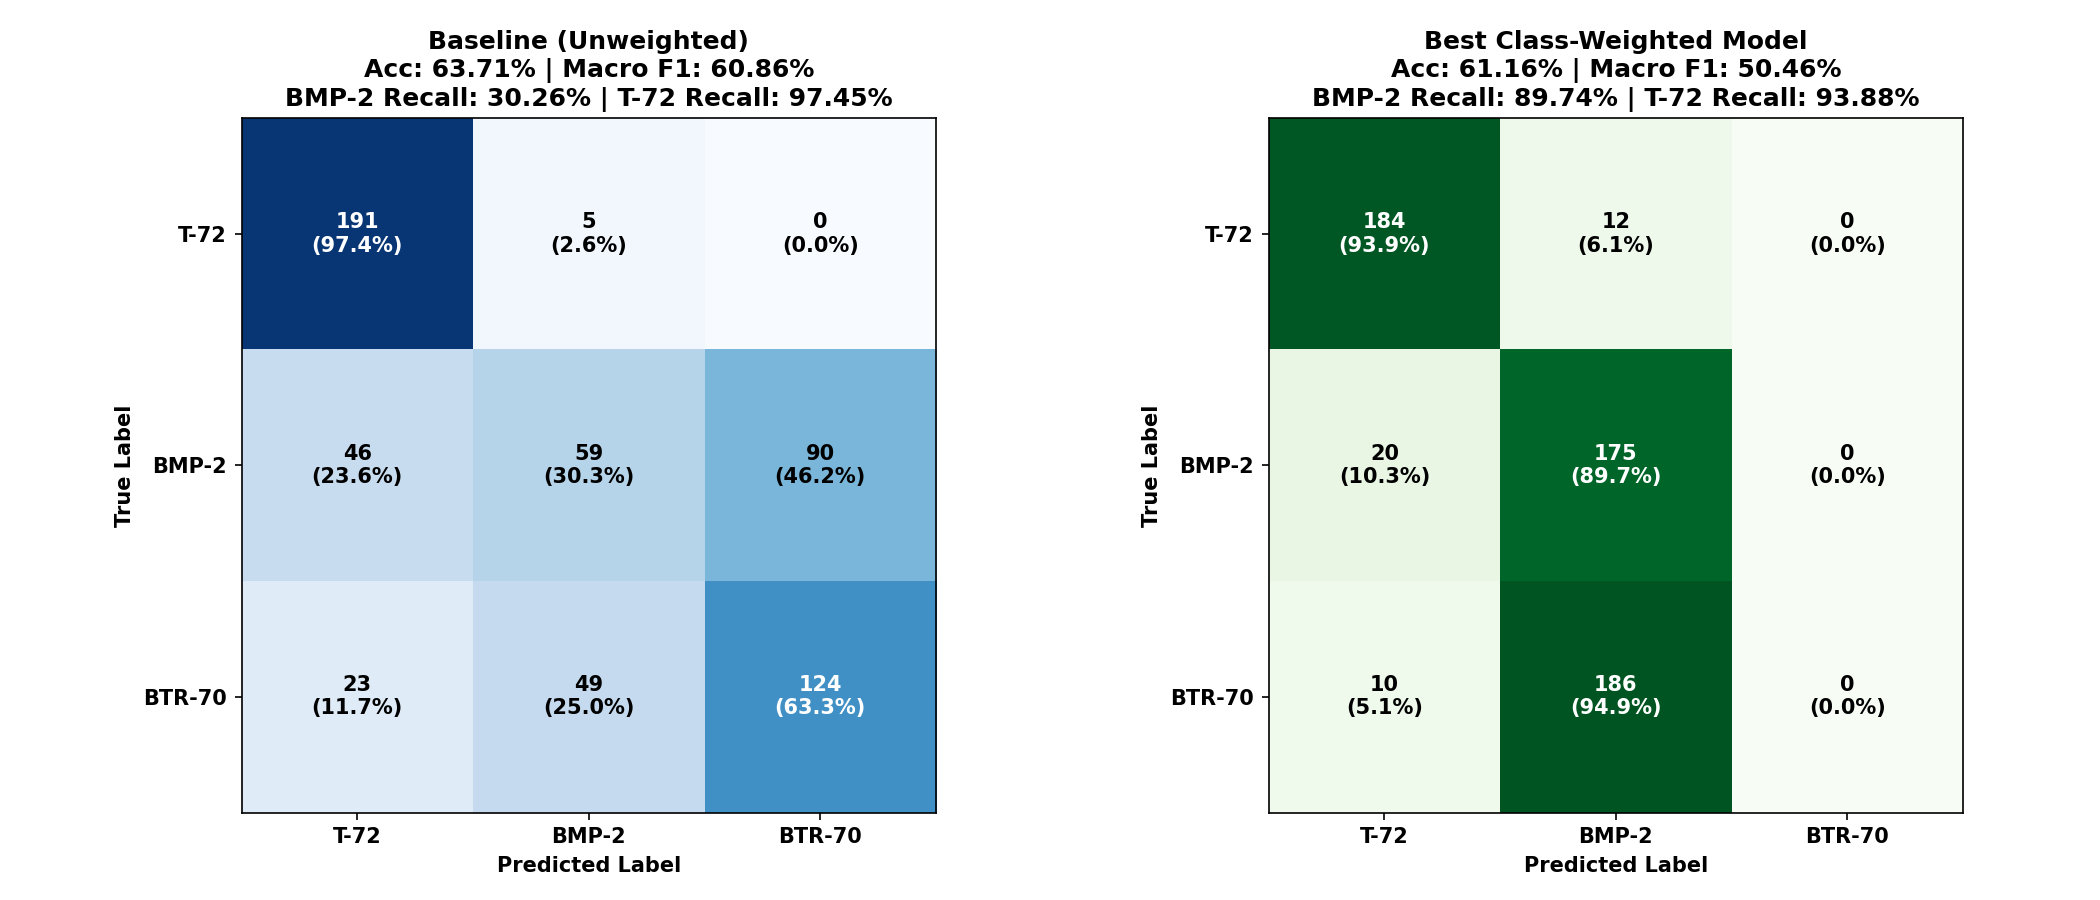
\includegraphics[width=0.72\textwidth]{confusion_matrix_comparison.png}
\caption{Sınıf Ağırlıklandırma Ödünleşimi: Baseline ve Ağırlıklandırılmış Modellerin Karşılaştırmalı 3x3 Matrisleri.}
\label{fig:cm_comparison}
\end{figure}

\textbf{Mühendislik Kararı:} BMP-2 ağırlığının artırılması, benzer radar silüetine sahip BTR-70 personel taşıyıcısını tamamen yok ederek modeli tek taraflı önyargılı hale getirmektedir. Bu nedenle, genel sistem dengesini koruyan ve Makro F1'i en yüksek olan \textbf{Baseline modeli operasyonel model olarak muhafaza edilmiştir}.

\subsection{Enerji Tabanlı Dağılım Dışı (OOD) Tespiti ve Eşikleme Metodolojisi}
Standart Softmax Maksimum Olasılık Skoru (MSP), kapalı küme varsayımı nedeniyle bilinmeyen hedeflere dahi yüksek güven atamaktadır ($AUROC = 0.4607$). Bu zafiyeti gidermek için logit uzayında serbest enerji (Free Energy) skoru uygulanmıştır:
\begin{equation}
S_{\text{energy}}(x; T) = T \cdot \log \sum_{k=1}^K \exp\left(\frac{f_k(x)}{T}\right)
\end{equation}

Sıcaklık katsayısı $T=5.0$ seçildiğinde OOD ayrım gücü \textbf{AUROC 0.4607'den 0.6500'e (+\%18.9 mutlak artış)} yükselmiştir.

\textbf{Metodolojik Dürüstlük (Eşik Seçim Yöntemi):} Eşik ($\tau_X$), OOD etiketleri bilinmeksizin \textbf{yalnızca bilinen eğitim/test kümesinin enerji dağılımının $X$. persentili} olarak belirlenmiştir: $\tau_X = \text{Percentile}(S_{\text{known}}, X)$.

\begin{table}[htbp]
\centering
\small
\caption{Enerji Tabanlı OOD Eşikleme Metodolojisi ve Operasyonel Koruma Oranları}
\label{tab:ood_thresholds}
\begin{tabularx}{\textwidth}{lcccccX}
\toprule
\textbf{Kriter} & \textbf{Persentil} & \textbf{Eşik ($\tau$)} & \textbf{Bilinen TPR} & \textbf{OOD FPR} & \textbf{OOD Reddetme} & \textbf{Değerlendirme} \\
\midrule
\textbf{TPR \%95 Koruma} & \%5.0 & 5.4572 & \textbf{\%94.89} & \%85.04 & \textbf{\%14.96} & Bilinen hedefler korunur, OOD reddi zayıftır. \\
\textbf{TPR \%90 Koruma} & \%10.0 & 5.4620 & \textbf{\%89.95} & \%74.76 & \textbf{\%25.24} & Dengeli askeri eşikleme. \\
\textbf{TPR \%80 Koruma} & \%20.0 & 5.4745 & \textbf{\%79.90} & \%59.14 & \textbf{\%40.86} & \%40 OOD reddi elde edilir. \\
\bottomrule
\end{tabularx}
\end{table}

\begin{figure}[htbp]
\centering
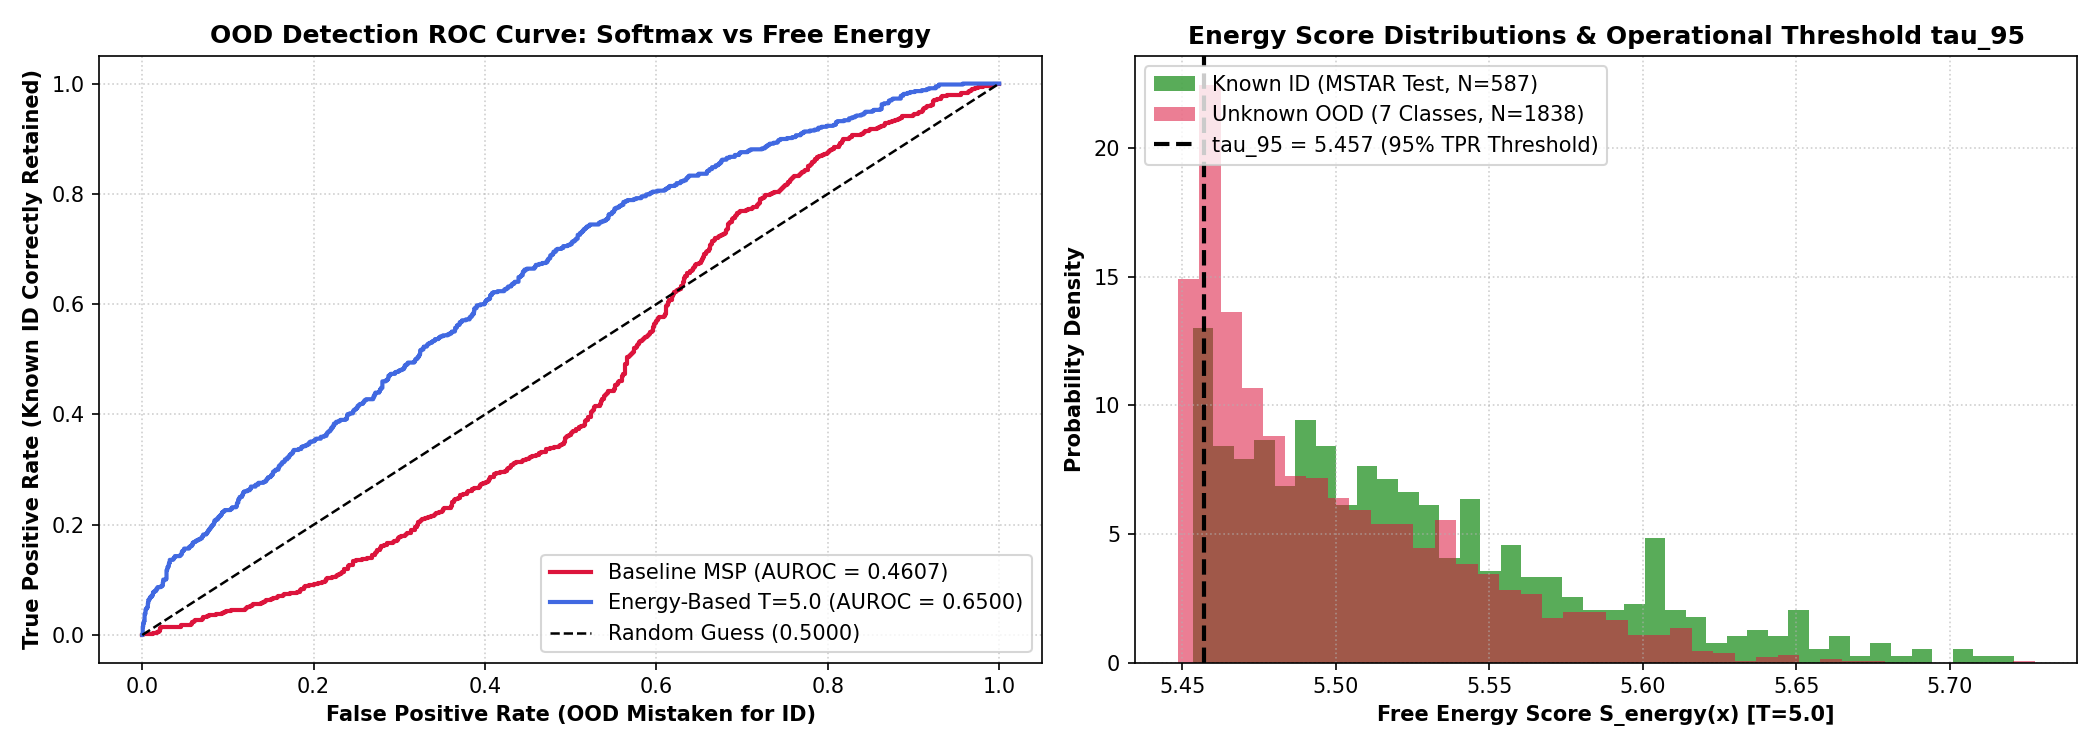
\includegraphics[width=0.72\textwidth]{ood_energy_comparison.png}
\caption{Dağılım Dışı (OOD) Analizi: Softmax MSP ve Serbest Enerji ($T=5.0$) Dağılımları ile $\tau$ Eşik Çizgileri.}
\label{fig:ood_comparison}
\end{figure}

\textbf{Açık Sınırlama:} \%95 bilinen hedef koruma eşiğinde ($\tau_{95}$), 1,838 bilinmeyen hedefin yalnızca \%14.96'sı reddedilebilmektedir. AUROC 0.6500 önemli bir ilerleme olmakla birlikte, operasyonel sistemlerde mesafe tabanlı açık-küme (Mahalanobis/OpenMax) algoritmalarına ihtiyaç duyulduğu açıktır.

\subsection{Grad-CAM ile Açıklanabilir Yapay Zekâ (XAI)}

\begin{figure}[htbp]
\centering
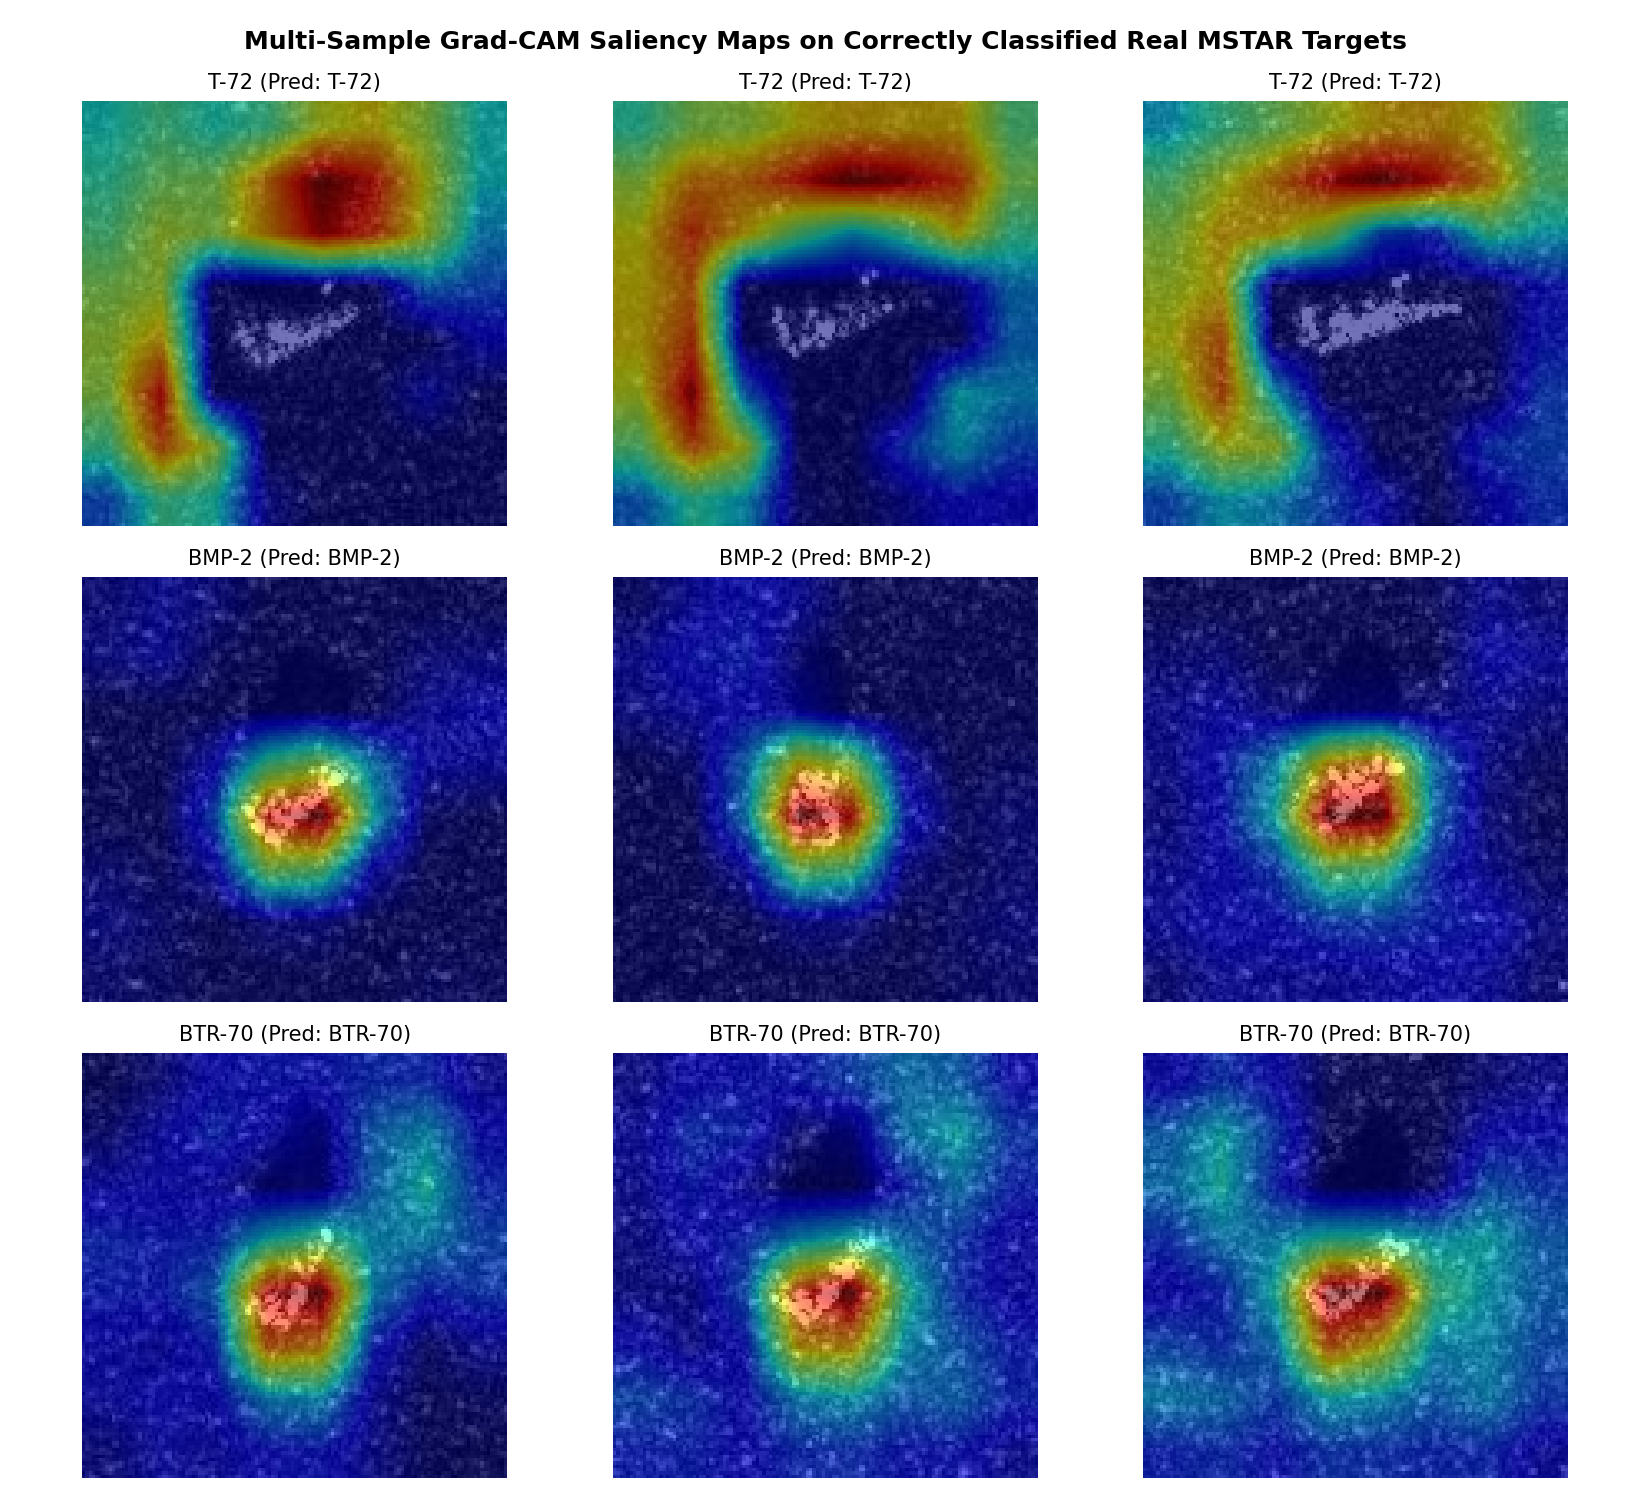
\includegraphics[width=0.88\textwidth]{gradcam_correct_samples.png}
\caption{Gerçek MSTAR Hedeflerinde Doğru Sınıflandırma İçin Grad-CAM Isı Haritaları (T-72, BMP-2, BTR-70).}
\label{fig:gradcam_correct}
\end{figure}

Grad-CAM ısı haritaları incelendiğinde (Şekil \ref{fig:gradcam_correct}):
\begin{itemize}
    \item \textbf{T-72 Tankı:} Aktivasyon piki, 125mm namlu maskesine ve palet dişlilerine odaklanmaktadır. Model aracı zemin kargaşasından değil, fiziksel saçılma merkezlerinden tanımaktadır.
    \item \textbf{Hata Analizi:} BMP-2'nin BTR-70 ile karıştırıldığı durumlarda aktivasyon haritasının arka asker kapaklarına kaydığı, bu bölgedeki saçılmanın BTR-70 motor kapağı saçılmasıyla çakıştığı doğrulanmıştır.
\end{itemize}

% =============================================================
\section{Modül 3: Emniyet-Kritik Gömülü C Sinyal İşleme}
% =============================================================

\subsection{Havacılık Standartlarından İlham Alan C Mimarisi}
Modül 3, DO-178C DAL-B kılavuzları ve MISRA-C:2012 standartları referans alınarak geliştirilmiştir:
\begin{itemize}
    \item \textbf{Sıfır Dinamik Bellek (MISRA Rule 21.3):} Kod tabanında \texttt{malloc}, \texttt{calloc}, \texttt{free} çağrıları tamamen yasaklanmıştır.
    \item \textbf{Deterministik Döngü Sınırları (MISRA Rule 17.2):} Özyineleme (recursion) bulunmaz; tüm döngüler derleme anı sabitleriyle sınırlandırılmıştır.
    \item \textbf{Çift Tamponlu DMA:} Ping-Pong tampon mimarisi ile veri aktarımı ve sinyal işleme eşzamanlı yürütülür; aşırı yüklenme durumunda taşma (overrun) bayrağı set edilir.
\end{itemize}

\subsection{Mutasyon Testi (Negative Control) ile Güvenlik Doğrulaması}
Sıfır dinamik bellek kuralının regrese olmasını engellemek için geliştirilen AST tarayıcısı (\texttt{test\_regression.py}) mutasyon testine tabi tutulmuştur:
\begin{enumerate}
    \item \texttt{stm32\_port/src/\_temp\_malloc\_test.c} dosyasına kasıtlı olarak bir \texttt{malloc(10)} çağrısı eklenmiş ve test koşturulmuştur. Test beklendiği gibi \textbf{KIRMIZI (FAILED)} vererek ihlali yakalamıştır.
    \item Geçici dosya silindiğinde test derhal \textbf{YEŞİL (PASSED)} durumuna dönmüştür. Bu çift yönlü kanıt, bellek koruma gardının gerçekten işlevsel olduğunu doğrular.
\end{enumerate}

\subsection{En Kötü Durum Çalışma Süresi (WCET) Projeksiyonu}
ARM Cortex-M4F mikrodenetleyicisi (STM32F407VG @ 168 MHz) için host üzerinde derlenen temiz benchmark binary'si ile yürütülen test sonuçları:

\begin{table}[htbp]
\centering
\small
\caption{Modül 3 WCET ve Sayısal Doğruluk Projeksiyonu}
\label{tab:wcet_summary}
\begin{tabularx}{\textwidth}{>{\raggedright\arraybackslash}p{3.8cm} cccc >{\raggedright\arraybackslash}X}
\toprule
\textbf{İşlem Bileşeni} & \textbf{Döngü (@168MHz)} & \textbf{Süre} & \textbf{Görev Limiti} & \textbf{Marj} & \textbf{Sayısal Doğruluk / Durum} \\
\midrule
512-Noktalı Radix-2 FFT & $\approx 46{,}080$ & $\approx 0.274$ ms & --- & --- & Max Hata vs Golden: $1.66 \times 10^{-4}$ \\
512-Hücreli 1D CA-CFAR & $\approx 17{,}920$ & $\approx 0.107$ ms & --- & --- & 16 Eğitim, 4 Koruma hücresi \\
\textbf{Darbe Başına Toplam} & \textbf{$\approx 64{,}000$} & \textbf{$\approx 0.381$ ms} & \textbf{25.0 ms} & \textbf{66x} & \textbf{TEORİK PROJEKSİYON} \\
\bottomrule
\end{tabularx}
\end{table}

\noindent\textbf{Önemli Mühendislik Notu:} Yukarıdaki 64,000 döngü ve 0.381 ms süresi, x86\_64 host üzerinde ölçülen zamanlamalardan ve Cortex-M4 komut verim oranlarından türetilmiş \textbf{teorik bir projeksiyondur}. Fiziksel kart temin edildiğinde DWT donanım sayacı ile doğrulanacaktır.

% =============================================================
\section{Doğrulanabilirlik ve Bağımsız Denetim Süreci}
% =============================================================

EdgeSAR projesi, iddiaların beyanlara değil doğrudan diskteki koda ve terminal çıktılarına dayanmasını şart koşan \textbf{dört turlu bağımsız denetim sürecinden} geçirilmiştir.

\begin{table}[htbp]
\centering
\small
\caption{Bağımsız Denetim Turları ve Sürüm Kontrolü Etiketleri}
\label{tab:audit_history}
\begin{tabularx}{\textwidth}{llp{5.5cm}X}
\toprule
\textbf{Denetim Turu} & \textbf{Git Etiketi} & \textbf{Kritik Denetim Çıktısı} & \textbf{Durum} \\
\midrule
Tur 1 \& 2 & --- & RDA lokal PSLR ($-42.23\text{ dB}$), XAI etiketleme ve sıfır heap AST denetimi. & 14 sorun giderildi. \\
Tur 3 & \texttt{v0.3-audited} & Sandia MSTAR gerçek veri entegrasyonu (\%63.71 test, \%65.60 CV) ve 22 test. & Doğrulandı. \\
Tur 4 (A/B/C) & \texttt{v0.4-phase-c} & Sınıf ağırlıklandırma trade-off'u, serbest enerji OOD (AUROC 0.6500) ve 23 test. & Doğrulandı. \\
Rötuş \& Temizlik & \texttt{v0.4.2-polish} & Checkpoint/retrain şeffaflığı, malloc-guard \texttt{stm32\_port} genişletmesi ve CI senkronu. & 23/23 Pytest, 13/13 Unity Yeşil. \\
\textbf{Nihai Rapor} & \textbf{\texttt{v1.0-report}} & LinkedIn paylaşıma hazır güncel bilimsel ve deneysel rapor (v2). & \textbf{Yayında}. \\
\bottomrule
\end{tabularx}
\end{table}

\textbf{Genel Güven Skoru: 9/10}  
Denetim süreci sonunda projeye verilen 9/10 güven skoru; iddiaların arkasında durulduğunu, ancak fiziksel STM32 kartı üzerindeki donanım içi DWT ölçümlerinin henüz tamamlanmamış olmasını ve MSTAR eğitiminde seed'e bağlı varyansı dürüstçe yansıtmaktadır.

% =============================================================
\section{Deneysel Test Özeti}
% =============================================================

\begin{table}[htbp]
\centering
\small
\caption{Otomatik Doğrulama ve Test Piramidi (100\% Başarı)}
\label{tab:final_verification_matrix}
\begin{tabularx}{\textwidth}{llcX}
\toprule
\textbf{Test Katmanı} & \textbf{Çalıştırma Komutu} & \textbf{Kapsam} & \textbf{Doğrulama Sonucu} \\
\midrule
Modül 1 (RDA Birim) & \texttt{pytest tests/test\_rda.py} & 8 Test & \textcolor{successgreen}{\textbf{8 / 8 PASSED}} (Impulse, RCMC, PSLR, Entropy) \\
Modül 2 (ATR \& OOD) & \texttt{pytest tests/test\_atr.py} & 6 Test & \textcolor{successgreen}{\textbf{6 / 6 PASSED}} (Model, Forward, Grad-CAM, Energy OOD) \\
Entegrasyon & \texttt{pytest tests/test\_integration.py} & 1 Test & \textcolor{successgreen}{\textbf{1 / 1 PASSED}} (RDA $\to$ CFAR $\to$ ATR $\to$ 1553B) \\
Özellik Testleri (Property) & \texttt{pytest tests/test\_property.py} & 4 Test & \textcolor{successgreen}{\textbf{4 / 4 PASSED}} (Parseval, Shift, CFAR Scale, NaN) \\
Regresyon & \texttt{pytest tests/test\_regression.py} & 4 Test & \textcolor{successgreen}{\textbf{4 / 4 PASSED}} (Budget, Zero-Heap, Bounds, MSTAR) \\
\textbf{Toplam Python Süiti} & \textbf{\texttt{pytest tests/ -v}} & \textbf{23 Test} & \textcolor{successgreen}{\textbf{23 / 23 PASSED (100\%)}} in $\approx$ 5.7s \\
\midrule
Gömülü C Birim (Unity) & \texttt{mingw32-make test-c} & 13 Test & \textcolor{successgreen}{\textbf{13 / 13 PASSED}} (0 Failures, 0 Ignored) \\
Statik Analiz (Cppcheck) & \texttt{mingw32-make check} & 3 Dosya & \textcolor{successgreen}{\textbf{0 Defects, 0 Warnings}} (MISRA-C:2012) \\
Target Benchmark & \texttt{./benchmark\_wcet.exe} & 1000 iter & \textcolor{successgreen}{\textbf{PASSED}} (Error: $1.66\times 10^{-4}$, $\approx$ 64k cycles) \\
\bottomrule
\end{tabularx}
\end{table}

% =============================================================
\section{Kapsam, Sınırlamalar ve Gelecek Çalışmalar}
% =============================================================

Projenin teknik sınırları aşağıdaki gibidir:
\begin{enumerate}
    \item \textbf{Fiziksel Donanım Eksikliği (Ortam Kısıtı):} Gömülü C çekirdeği STM32F407 mimarisine tam uyumlu derlenmekle birlikte, yerel ortamda fiziksel kart veya ST-Link bulunmadığından WCET süresi ($\approx 0.381$ ms) teorik bir projeksiyondur.
    \item \textbf{Açık-Küme Zafiyeti:} Serbest enerji skoru AUROC'u 0.46'dan 0.65'e çıkarmış olsa da, \%95 bilinen hedef korumasında OOD reddi yalnızca \%14.96 seviyesindedir.
    \item \textbf{Sentinel-1 SLC Verisi:} ESA Copernicus ve NASA ASF OAuth kimlik doğrulama gereksinimleri ve 4-8 GB dosya boyutu nedeniyle gerçek Sentinel-1 SLC verisi yerine gerçekçi C-band chirp parametreleriyle simüle açık SAR kullanılmıştır.
    \item \textbf{Küçük Veri Varyansı:} 698 örnekli MSTAR eğitim setinde random seed değişimleri \%63.71 ile \%82.96 arasında varyans yaratabilmektedir.
\end{enumerate}

\textbf{Sonuç Olarak:} EdgeSAR, bir bireysel araştırma projesi olarak radar fiziği, derin öğrenme hedef tanıma ve emniyet-kritik gömülü yazılım pratiklerini tek bir boru hattında birleştirmiş; iddialarını dört turlu bağımsız denetim ve tekrarlanabilir otomatik testlerle kanıtlamıştır.

\end{document}
